\chapter{引言}
\label{cha:intro}
UNIX~操作系统(UNIX),是美国AT\&T公司1971年~在PDP-11上运行的操作系统。具有多用户、
多任务的特点,支持多种处理器架构,最早由肯·湯普遜(Kenneth Lane Thompson)、
丹尼斯·里奇(Dennis MacAlistair Ritchie),见图\ref{fig:ken}。和~Douglas
McIlroy~于1969年在~AT\&T~的贝尔实验室开发\footnote{摘自中文维基百科}。\par
\begin{figure}[htbp]
    \centering
	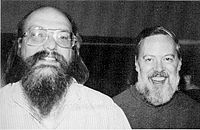
\includegraphics{Ken_n_dennis}
    \caption{肯·汤普逊(左)和丹尼斯·里奇(右)}
    \label{fig:ken}
\end{figure}
Linux~操作系统(Linux),是一类计算机操作系统的统称。Linux~操作系统的内核的名字也是~“Linux”。
Linux~操作系统也是自由软件和开放源代码发展中最著名的例子。严格来讲,Linux~这个词本身只表
示~Linux~内核,但在实际上人们已经习惯了用~Linux~来形容整个基于~Linux~内核,并且使用~GNU~
工程各种工具和数据库的操作系统(也被称为~GNU/Linux~)。基于这些组
件的~Linux~软件被称为~Linux~发行版。

Linux内核最初只是由芬兰人林纳斯·托瓦兹(Linus
Torvalds),见图\ref{fig:linus},在赫尔辛基大学上学时出于
个人爱好而编写的,当时他并不满意~Minix~这个教学用的操作系统,部分因为只能在有限硬件上运行。
最初的设想中,Linux~是一种类似~Minix~这样的一种操作系统。Linux~的第一个版本在1991年9月
被大学~FTP server~管理员~Ari Lemmke~发布在~Internet~上,最初~Torvalds~称这个内核的名称为
~"Freax",意思是自由("free")和奇异("freak")的结合字,并且
附上了~"X"~这个常用的字母,以配合所谓的~Unix-like~的系统。但是~FTP server~管理员
嫌原来的命名~“Freax”~的名称不好听,把内核的称呼改成~“Linux”~,当时仅有10000行代码,仍必须
运行于~Minix~操作系统之上,并且必须使用硬盘开机;随后在10月份第二个版本(0.02版)
就发布了,同时这位芬兰赫尔辛基的大学生在~comp.os.minix~上发布一则消息\par
\begin{center}
\fbox{\parbox[t]{0.8\textwidth}{
Hello everybody out there using minix-\\
I'm doing a (free) operation system (just a hobby,\\
won't be big and professional like gnu) for 386(486) AT clones.}}
\end{center}
\begin{figure}[htbp]
    \centering
    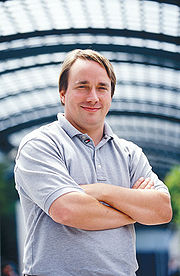
\includegraphics{Linus_Torvalds}
    \caption{Linus Torvalds}
    \label{fig:linus}
\end{figure}

\section{UNIX~历史}
\label{sec:history}
UNIX~的历史开始于1969年~ken Thompson,Dennis Ritchie~(即著名的~K\&G~,~C~语言的发明人)
与一群人在一部~PDP-7~上进行的一些工作,后来这个系统变成了~UNIX。\par
主要大事件:
\begin{itemize}
    \item V1(1971):第一版的UNIX,以~PDP-11/20的汇编语言写成。
        包括文件系统,~fork、roff、ed~等软件。
    \item V4(1973):以~C~语言从头写过,这使得~UNIX~修改容易,可以在几个月内移
        植到新的硬件平台上。最初C语言是为~UNIX~设计的,所以~C~与~UNIX~间有紧密的关系。
    \item V6(1975):第一个在贝尔实验室外(尤其是大学中)广为流传的~UNIX~版本。
        这也是~UNIX~分支的起点与广受欢迎的开始。1.xBSD (PDP-II)就是由这个版本衍生出来的。
    \item V7(1979):在许多UNIX玩家的心目中,这是“最后一个真正的~UNIX,”
        这个版本包括一个完整的~K\&RC~编译器,Bourne
        shell。V7~移植到~VAX~机器后称为~32V。
\end{itemize}
\section{UNIX~家谱}
目前开发~UNIX(System V)的公司是~Unix System Laboratories
(USL)。USL~本为~AT\&T~所有,1993年初被~Novell~收购。Novell~于1993年末将~UNIX~这个注册商标
转让给~X/Open~组织。

\label{sec:family}

详细的~UNIX~编年史\url{http://www.levenez.com/unix/}。

\section{表格样本}
\label{chap1:sample:table}

\subsection{基本表格}
\label{sec:basictable}

模板中关于表格的宏包有三个: \textsf{booktabs}、\textsf{array} 和
\textsf{longtabular},命令有一个 \verb|\hlinewd|。三线表可以用 \textsf{booktabs}
提供的 \verb|\toprule|、\verb|\midrule| 和 \verb|\bottomrule|。它们与
\textsf{longtable} 能很好的配合使用。如果表格比较简单的话可以直接用命令
\verb|hlinewd{xpt}| 控制。
\begin{table}[htb]
  \centering
  \begin{minipage}[t]{0.8\linewidth} % 如果想在表格中使用脚注,minipage是个不错的办法
  \caption[模板文件]{模板文件。如果表格的标题很长,那么在表格索引中就会很不美
    观,所以要像 chapter 那样在前面用中括号写一个简短的标题。这个标题会出现在索
    引中。}
  \label{tab:template-files}
    \begin{tabular*}{\linewidth}{lp{10cm}}
      \toprule[1.5pt]
      {\heiti 文件名} & {\heiti 描述} \\\midrule[1pt]
      tongjithesis.cls & 模板类文件。\footnote{表格中的脚注}\\
      tongjithesis.cfg & 模板配置文件\footnote{再来一个}。\\
      tongjibib.bst    & 参考文献 Bibtex 样式文件。\\
      tongjitils.sty   & 常用的包和命令写在这里,减轻主文件的负担。\\
       shuji.tex & 书脊示例文档\\
 ref/ & 示例文档参考文献目录\\
 data/ & 示例文档章节具体内容\\
 figures/ & 示例文档图片路径\\
 tongjitils.sty & 为示例文档加载其它宏包\\\hline
 \textbf{TongjiThesisReadme.pdf} & 用户手册(本文档)\\
      \bottomrule[1.5pt]
    \end{tabular*}
  \end{minipage}
\end{table}



首先来看一个最简单的表格。表 \ref{tab:template-files} 列举了本模板主要文件及其功
能。请大家注意三线表中各条线对应的命令。这个例子还展示了如何在表格中正确使用脚注。
由于 \LaTeX{} 本身不支持在表格中使用 \verb|\footnote|,所以我们不得不将表格放在
小页中,而且最好将表格的宽度设置为小页的宽度,这样脚注看起来才更美观。

\subsection{表格下方标注数据来源}
\label{sec:tabsource}

我们经常会在表格下方标注数据来源,或者对表格里面的条目进行解释。前面的脚注是一种
不错的方法,如果你不喜欢脚注。那么完全可以在表格后面自己写注释,比如表~\ref{tab:tabexamp1}。
\begin{table}[h]
  \centering
  \caption{复杂表格示例 1}
  \label{tab:tabexamp1}
  \begin{minipage}[t]{0.8\textwidth}
    \begin{tabularx}{\linewidth}{|l|X|X|X|X|}
      \hline
 \multirow{2}*{\backslashbox{x}{y}}  & \multicolumn{2}{c|}{First Half} & \multicolumn{2}{c|}{Second Half}\\\cline{2-5}
      & 1st Qtr &2nd Qtr&3rd Qtr&4th Qtr \\ \hline
      East$^{*}$ &   20.4&   27.4&   90&     20.4 \\
      West$^{**}$ &   30.6 &   38.6 &   34.6 &  31.6 \\ \hline
    \end{tabularx}\\[2pt]
    \footnotesize 注:数据来源《\tongjithesis{} 使用手册》。\\
    *:东部\\
    **:西部
  \end{minipage}
\end{table}

此外,表~\ref{tab:tabexamp1} 同时还演示了另外两个功能:1)通过 \textsf{tabularx} 的
 \texttt{|X|} 扩展实现表格自动放大;2)通过命令 \verb|\backslashbox| 在表头部分
插入反斜线。

为了使我们的例子更接近实际情况,我会在必要的时候插入一些“无关”文字,以免太多图
表同时出现,导致排版效果不太理想。第一个出场的当然是我的最爱:风流潇洒、骏马绝尘、
健笔凌云的{\heiti 李太白}了。

李白,字太白,陇西成纪人。凉武昭王暠九世孙。或曰山东人,或曰蜀人。白少有逸才,志
气宏放,飘然有超世之心。初隐岷山,益州长史苏颋见而异之,曰:“是子天才英特,可比
相如。”天宝初,至长安,往见贺知章。知章见其文,叹曰:“子谪仙人也。”言于明皇,
召见金銮殿,奏颂一篇。帝赐食,亲为调羹,有诏供奉翰林。白犹与酒徒饮于市,帝坐沉香
亭子,意有所感,欲得白为乐章,召入,而白已醉。左右以水颒面,稍解,援笔成文,婉丽
精切。帝爱其才,数宴见。白常侍帝,醉,使高力士脱靴。力士素贵,耻之,摘其诗以激杨
贵妃。帝欲官白,妃辄沮止。白自知不为亲近所容,恳求还山。帝赐金放还。乃浪迹江湖,
终日沉饮。永王璘都督江陵,辟为僚佐。璘谋乱,兵败,白坐长流夜郎,会赦得还。族人阳
冰为当涂令,白往依之。代宗立,以左拾遗召,而白已卒。文宗时,诏以白歌诗、裴旻剑舞、
张旭草书为三绝云。集三十卷。今编诗二十五卷。\hfill\pozhehao《全唐诗》诗人小传

\subsection{浮动体的并排放置}
浮动体的并排放置一般有两种情况:1)二者没有关系,为两个独立的浮动体;2)二者隶属
于同一个浮动体。对表格来说并排表格既可以像表~\ref{tab:parallel1}、表~\ref{tab:parallel2}
使用小页环境,也可以如表~\ref{tab:subtable} 使用子表格来做。图的例子参见第~\ref{sec:multifig} 节。
\begin{table}[h]
\noindent\begin{minipage}{0.5\textwidth}
\centering
\caption{第一个并排子表格}
\label{tab:parallel1}
\begin{tabular}{p{2cm}p{2cm}}
\toprule[1.5pt]
111 & 222 \\\midrule[1pt]
222 & 333 \\\bottomrule[1.5pt]
\end{tabular}
\end{minipage}
\begin{minipage}{0.5\textwidth}
\centering
\caption{第二个并排子表格}
\label{tab:parallel2}
\begin{tabular}{p{2cm}p{2cm}}
\toprule[1.5pt]
111 & 222 \\\midrule[1pt]
222 & 333 \\\bottomrule[1.5pt]
\end{tabular}
\end{minipage}
\end{table}

然后就是忧国忧民,诗家楷模杜工部了。杜甫,字子美,其先襄阳人,曾祖依艺为巩令,因
居巩。甫天宝初应进士,不第。后献《三大礼赋》,明皇奇之,召试文章,授京兆府兵曹参
军。安禄山陷京师,肃宗即位灵武,甫自贼中遁赴行在,拜左拾遗。以论救房琯,出为华州
司功参军。关辅饥乱,寓居同州同谷县,身自负薪采梠,餔糒不给。久之,召补京兆府功曹,
道阻不赴。严武镇成都,奏为参谋、检校工部员外郎,赐绯。武与甫世旧,待遇甚厚。乃于
成都浣花里种竹植树,枕江结庐,纵酒啸歌其中。武卒,甫无所依,乃之东蜀就高適。既至
而適卒。是岁,蜀帅相攻杀,蜀大扰。甫携家避乱荆楚,扁舟下峡,未维舟而江陵亦乱。乃
溯沿湘流,游衡山,寓居耒阳。卒年五十九。元和中,归葬偃师首阳山,元稹志其墓。天宝
间,甫与李白齐名,时称李杜。然元稹之言曰:“李白壮浪纵恣,摆去拘束,诚亦差肩子美
矣。至若铺陈终始,排比声韵,大或千言,次犹数百,词气豪迈,而风调清深,属对律切,
而脱弃凡近,则李尚不能历其藩翰,况堂奥乎。”白居易亦云:“杜诗贯穿古今,  尽工尽
善,殆过于李。”元、白之论如此。盖其出处劳佚,喜乐悲愤,好贤恶恶,一见之于诗。而
又以忠君忧国、伤时念乱为本旨。读其诗可以知其世,故当时谓之“诗史”。旧集诗文共六
十卷,今编诗十九卷。

\begin{table}
\centering
\caption{并排子表格}
\label{tab:subtable}
\subcaptionbox{第一个子表格}
{
  \begin{tabular}{p{2cm}p{2cm}}
  \toprule[1.5pt]
  111 & 222 \\\midrule[1pt]
  222 & 333 \\\bottomrule[1.5pt]
  \end{tabular}
}
\hskip2cm
\subcaptionbox{第二个子表格}
{
  \begin{tabular}{p{2cm}p{2cm}}
  \toprule[1.5pt]
  111 & 222 \\\midrule[1pt]
  222 & 333 \\\bottomrule[1.5pt]
  \end{tabular}
}
\end{table}

\subsection{非常复杂非常漂亮的表格}
不可否认 \LaTeX{} 的表格功能没有想象中的那么强大,不过只要你足够认真,足够细致,那么
同样可以排出来非常复杂非常漂亮的表格。请参看表~\ref{tab:tabexamp2}。
\begin{table}[hb]
  \centering\dawu[1.3]
  \caption{复杂表格示例 2}
  \label{tab:tabexamp2}
  \begin{tabular}[c]{|c|m{0.8in}|c|c|c|c|c|}\hline
    \multicolumn{2}{|c|}{Network Topology} & \# of nodes &
    \multicolumn{3}{c|}{\# of clients} & Server \\\hline
    GT-ITM & Waxman Transit-Stub & 600 &
    \multirow{2}{2em}{2\%}&
    \multirow{2}{2em}{10\%}&
    \multirow{2}{2em}{50\%}&
    \multirow{2}{1.2in}{Max. Connectivity}\\\cline{1-3}
    \multicolumn{2}{|c|}{Inet-2.1} & 6000 & & & &\\\hline
    \multirow{2}{1in}{Xue} & Rui  & Ni &\multicolumn{4}{c|}{\multirow{2}*{\tongjithesis}}\\\cline{2-3}
    & \multicolumn{2}{c|}{ABCDEF} &\multicolumn{4}{c|}{} \\\hline
\end{tabular}
\end{table}

最后就是清新飘逸、文约意赅、空谷绝响的王大侠了。王维,字摩诘,河东人。工书画,与
弟缙俱有俊才。开元九年,进士擢第,调太乐丞。坐累为济州司仓参军,历右拾遗、监察御
史、左补阙、库部郎中,拜吏部郎中。天宝末,为给事中。安禄山陷两都,维为贼所得,服
药阳喑,拘于菩提寺。禄山宴凝碧池,维潜赋诗悲悼,闻于行在。贼平,陷贼官三等定罪,
特原之,责授太子中允,迁中庶子、中书舍人。复拜给事中,转尚书右丞。维以诗名盛于开
元、天宝间,宁薛诸王驸马豪贵之门,无不拂席迎之。得宋之问辋川别墅,山水绝胜,与道
友裴迪,浮舟往来,弹琴赋诗,啸咏终日。笃于奉佛,晚年长斋禅诵。一日,忽索笔作书
数纸,别弟缙及平生亲故,舍笔而卒。赠秘书监。宝应中,代宗问缙:“朕常于诸王坐闻维
乐章,今存几何?”缙集诗六卷,文四卷,表上之。敕答云,卿伯氏位列先朝,名高希代。
抗行周雅,长揖楚辞。诗家者流,时论归美。克成编录,叹息良深。殷璠谓维诗词秀调雅,
意新理惬。在泉成珠,著壁成绘。苏轼亦云:“维诗中有画,画中有诗也。”今编诗四卷。

要想用好论文模板还是得提前学习一些 \TeX/\LaTeX{}的相关知识,具备一些基本能力,掌
握一些常见技巧,否则一旦遇到问题还真是比较麻烦。我们见过很多这样的同学,一直以来
都是使用 Word 等字处理工具,以为 \LaTeX{}模板的用法也应该类似,所以就沿袭同样的思
路来对待这种所见非所得的排版工具,结果被折腾的焦头烂额,疲惫不堪。

\subsection{续表 :表格长度超过一页}
如果您要排版的表格长度超过一页,那么推荐使用 \textsf{longtable} 或者 \textsf{supertabular}
宏包,模板对 \textsf{longtable} 进行了相应的设置,所以用起来可能简单一些。
表~\ref{tab:performance} 就是 \textsf{longtable} 的简单示例。
\begin{longtable}[c]{c*{6}{r}}
\caption{实验数据}\label{tab:performance}\\
\toprule[1.5pt]
 测试程序 & \multicolumn{1}{c}{正常运行} & \multicolumn{1}{c}{同步} & \multicolumn{1}{c}{检查点} & \multicolumn{1}{c}{卷回恢复}
& \multicolumn{1}{c}{进程迁移} & \multicolumn{1}{c}{检查点} \\
& \multicolumn{1}{c}{时间 (s)}& \multicolumn{1}{c}{时间 (s)}&
\multicolumn{1}{c}{时间 (s)}& \multicolumn{1}{c}{时间 (s)}& \multicolumn{1}{c}{
  时间 (s)}&  文件(KB)\\\midrule[1pt]
\endfirsthead
\multicolumn{7}{c}{续表~\thetable\hskip1em 实验数据}\\
\toprule[1.5pt]
 测试程序 & \multicolumn{1}{c}{正常运行} & \multicolumn{1}{c}{同步} & \multicolumn{1}{c}{检查点} & \multicolumn{1}{c}{卷回恢复}
& \multicolumn{1}{c}{进程迁移} & \multicolumn{1}{c}{检查点} \\
& \multicolumn{1}{c}{时间 (s)}& \multicolumn{1}{c}{时间 (s)}&
\multicolumn{1}{c}{时间 (s)}& \multicolumn{1}{c}{时间 (s)}& \multicolumn{1}{c}{
  时间 (s)}&  文件(KB)\\\midrule[1pt]
\endhead
\hline
\multicolumn{7}{r}{续下页}
\endfoot
\endlastfoot
CG.A.2 & 23.05 & 0.002 & 0.116 & 0.035 & 0.589 & 32491 \\
CG.A.4 & 15.06 & 0.003 & 0.067 & 0.021 & 0.351 & 18211 \\
CG.A.8 & 13.38 & 0.004 & 0.072 & 0.023 & 0.210 & 9890 \\
CG.B.2 & 867.45 & 0.002 & 0.864 & 0.232 & 3.256 & 228562 \\
CG.B.4 & 501.61 & 0.003 & 0.438 & 0.136 & 2.075 & 123862 \\
CG.B.8 & 384.65 & 0.004 & 0.457 & 0.108 & 1.235 & 63777 \\
MG.A.2 & 112.27 & 0.002 & 0.846 & 0.237 & 3.930 & 236473 \\
MG.A.4 & 59.84 & 0.003 & 0.442 & 0.128 & 2.070 & 123875 \\
MG.A.8 & 31.38 & 0.003 & 0.476 & 0.114 & 1.041 & 60627 \\
MG.B.2 & 526.28 & 0.002 & 0.821 & 0.238 & 4.176 & 236635 \\
MG.B.4 & 280.11 & 0.003 & 0.432 & 0.130 & 1.706 & 123793 \\
MG.B.8 & 148.29 & 0.003 & 0.442 & 0.116 & 0.893 & 60600 \\
LU.A.2 & 2116.54 & 0.002 & 0.110 & 0.030 & 0.532 & 28754 \\
LU.A.4 & 1102.50 & 0.002 & 0.069 & 0.017 & 0.255 & 14915 \\
LU.A.8 & 574.47 & 0.003 & 0.067 & 0.016 & 0.192 & 8655 \\
LU.B.2 & 9712.87 & 0.002 & 0.357 & 0.104 & 1.734 & 101975 \\
LU.B.4 & 4757.80 & 0.003 & 0.190 & 0.056 & 0.808 & 53522 \\
LU.B.8 & 2444.05 & 0.004 & 0.222 & 0.057 & 0.548 & 30134 \\
EP.A.2 & 123.81 & 0.002 & 0.010 & 0.003 & 0.074 & 1834 \\
EP.A.4 & 61.92 & 0.003 & 0.011 & 0.004 & 0.073 & 1743 \\
EP.A.8 & 31.06 & 0.004 & 0.017 & 0.005 & 0.073 & 1661 \\
EP.B.2 & 495.49 & 0.001 & 0.009 & 0.003 & 0.196 & 2011 \\
EP.B.4 & 247.69 & 0.002 & 0.012 & 0.004 & 0.122 & 1663 \\
EP.B.8 & 126.74 & 0.003 & 0.017 & 0.005 & 0.083 & 1656 \\
CG.A.2 & 23.05 & 0.002 & 0.116 & 0.035 & 0.589 & 32491 \\
CG.A.4 & 15.06 & 0.003 & 0.067 & 0.021 & 0.351 & 18211 \\
CG.A.8 & 13.38 & 0.004 & 0.072 & 0.023 & 0.210 & 9890 \\
CG.B.2 & 867.45 & 0.002 & 0.864 & 0.232 & 3.256 & 228562 \\
CG.B.4 & 501.61 & 0.003 & 0.438 & 0.136 & 2.075 & 123862 \\
CG.B.8 & 384.65 & 0.004 & 0.457 & 0.108 & 1.235 & 63777 \\
MG.A.2 & 112.27 & 0.002 & 0.846 & 0.237 & 3.930 & 236473 \\
MG.A.4 & 59.84 & 0.003 & 0.442 & 0.128 & 2.070 & 123875 \\
MG.A.8 & 31.38 & 0.003 & 0.476 & 0.114 & 1.041 & 60627 \\
MG.B.2 & 526.28 & 0.002 & 0.821 & 0.238 & 4.176 & 236635 \\
MG.B.4 & 280.11 & 0.003 & 0.432 & 0.130 & 1.706 & 123793 \\
MG.B.8 & 148.29 & 0.003 & 0.442 & 0.116 & 0.893 & 60600 \\
LU.A.2 & 2116.54 & 0.002 & 0.110 & 0.030 & 0.532 & 28754 \\
LU.A.4 & 1102.50 & 0.002 & 0.069 & 0.017 & 0.255 & 14915 \\
LU.A.8 & 574.47 & 0.003 & 0.067 & 0.016 & 0.192 & 8655 \\
LU.B.2 & 9712.87 & 0.002 & 0.357 & 0.104 & 1.734 & 101975 \\
LU.B.4 & 4757.80 & 0.003 & 0.190 & 0.056 & 0.808 & 53522 \\
LU.B.8 & 2444.05 & 0.004 & 0.222 & 0.057 & 0.548 & 30134 \\
EP.A.2 & 123.81 & 0.002 & 0.010 & 0.003 & 0.074 & 1834 \\
EP.A.4 & 61.92 & 0.003 & 0.011 & 0.004 & 0.073 & 1743 \\
EP.A.8 & 31.06 & 0.004 & 0.017 & 0.005 & 0.073 & 1661 \\
EP.B.2 & 495.49 & 0.001 & 0.009 & 0.003 & 0.196 & 2011 \\
EP.B.4 & 247.69 & 0.002 & 0.012 & 0.004 & 0.122 & 1663 \\
EP.B.8 & 126.74 & 0.003 & 0.017 & 0.005 & 0.083 & 1656 \\
\bottomrule[1.5pt]
\end{longtable}

表~\ref{tab:data}~为采用\textsf{supertabular}实现长表格功能的示例。
\begin{center} \tablecaption{电容、电感以及电阻元件不确定时系统鲁棒稳定裕度参数 \label{tab:data}}
\tablefirsthead{
\toprule
\multicolumn{1}{c}{T$\left(^{\circ}C\right)$} &
\multicolumn{1}{c}{ $\gamma_C$}  &
\multicolumn{1}{c}{ $\gamma_L$}  &
\multicolumn{1}{c}{ $\gamma_R$} \\}
\tablehead{\multicolumn{4}{c}{\small 续表 \ref{tab:data}~电容、电感以及电阻元件不确定时系统鲁棒稳定裕度参数}\\
\bottomrule
\multicolumn{1}{c}{T$\left(^{\circ}C\right)$} &
\multicolumn{1}{c}{ $\gamma_C$}  &
\multicolumn{1}{c}{ $\gamma_L$}  &
\multicolumn{1}{c}{ $\gamma_R$} \\
\bottomrule}
\tabletail{\bottomrule
\multicolumn{2}{c}{\small 接下页} \\}
\tablelasttail{\bottomrule}
\begin{supertabular}{C{3cm}C{3cm}C{3cm}C{3cm}}
 \midrule
        $-60$                      & $0.8295$              & $0.7854$             & $0.9011$      \\

        $-50$                      & $0.8189$              & $0.7754$             & $0.9011$       \\

        $-40$                      & $0.8096$              & $0.7651$             & $0.9010$      \\

        $-30$                      & $0.7995$              & $0.7547$             & $0.9009$       \\

        $-20$                      & $0.7896$              & $0.7444$             & $0.9009$       \\

        $-10$                      & $0.7800$              & $0.7345$             & $0.9008$       \\

        $0$                         & $0.7707$              & $0.7248$             & $0.9008$        \\

        $10$                      & $0.7617$              & $0.7155$             & $0.9008$         \\

        $20$                      & $0.7529$              & $0.7063$             & $0.9007$       \\

        $30$                      & $0.7442$              & $0.6972$             & $0.9007$       \\

        $40$                      & $0.7356$              & $0.6881$             & $0.9007$      \\

        $50$                      & $0.7269$              & $0.6789$             & $0.9007$       \\

        $60$                      & $0.7182$              & $0.6697$             & $0.9007$       \\

        $70$                      & $0.7095$              & $0.6605$             & $0.9006$       \\

        $80$                      & $0.7009$              & $0.6514$             & $0.9006$       \\

        $90$                      & $0.6925$              & $0.6425$             & $0.9006$      \\

        $100$                    & $0.6846$              & $0.6340$             & $0.9006$       \\

        $110$                    & $0.6774$              & $0.6263$             & $0.9006$      \\

        $120$                    & $0.6711$              & $0.6196$             & $0.9006$      \\

        $130$                    & $0.6659$              & $0.6140$             & $0.9006$       \\

        $140$                    & $0.6621$              & $0.6100$             & $0.9005$       \\

        $150$                    & $0.6599$              & $0.6076$             & $0.9005$       \\

        $160$                    & $0.6594$              & $0.6070$             & $0.9005$       \\

        $170$                    & $0.6606$              & $0.6083$             & $0.9005$       \\

        $180$                    & $0.6634$              & $0.6113$             & $0.9006$       \\

        $190$                    & $0.6676$              & $0.6158$             & $0.9006$       \\

        $200$                    & $0.6729$              & $0.6215$             & $0.9006$       \\

        $210$                    & $0.6789$              & $0.6279$             & $0.9006$       \\

        $220$                    & $0.6848$              & $0.6342$             & $0.9006$       \\

        $230$                    & $0.6902$              & $0.6400$             & $0.9006$      \\

        $240$                    & $0.6945$              & $0.6446$             & $0.9006$       \\

        $250$                    & $0.6978$              & $0.6480$             & $0.9006$       \\

        $260$                    & $0.7006$              & $0.6511$             & $0.9006$       \\

        $270$                    & $0.7050$              & $0.6557$             & $0.9006$      \\

        $280$                    & $0.7148$              & $0.6661$             & $0.9006$      \\
\end{supertabular}
\end{center}

\subsection{设置每列的对齐格式以及宽度}
表~\ref{tab:chap1:IPM_function}使用新定义的\texttt{columntype}设置每列的对齐格式以及宽度。


泉眼无声惜细流,树阴照水爱晴柔。
小荷才露尖尖角,早有蜻蜓立上头。
试问世界上有这么好的诗么?
\begin{verbatim}
门前大桥下
游过一群鸭
快来快来数一数
二四六七八
嘎嘎嘎嘎
真呀真多呀
\end{verbatim}

\begin{table}[h]
\centering
\caption{IPM~智能功率模块引脚功能列表}
\label{tab:chap1:IPM_function}
\begin{tabular}{C{3.6cm}L{1.8cm}L{7.2cm}}
\toprule
\textbf{序号} & \textbf{名称} & \textbf{说明} \\
\midrule
1      & $U_P$   & $U_P$~相控制信号输入端子            \\
2      & $V_{P1}$  & $U_P$~相控制电源端子              \\
3      & $V_{UFB}$ & $U_P$~相驱动电源端子              \\
4      & $V_{UFS}$ & $U_P$~相驱动电源~GND~端子           \\
5      & $V_P$   & $V_P$~相控制信号输入端子            \\
6      & $V_{P1}$  & $V_P$相控制电源端子              \\
7      & $V_{VFB}$ & $V_P$相驱动电源端子              \\
8      & $V_{VFS}$ & $V_P$相驱动电源~GND~端子           \\
9      & $W_P$   & $W_P$~相控制信号输入端子            \\
10     & $V_{P1}$  & $W_P$~相控制电源端子              \\
11     & $V_{PC}$  & $U,V,W$~相控制电源GND端子       \\
12     & $V_{WFB}$ & $W_P$~相驱动电源端子              \\
13     & $V_{WFS}$ & $W_P$~相驱动电源GND端子           \\
14     & $V_{N1}$  & N~侧控制电源端子               \\
15     & $V_{NC}$  & N~侧控制电源~GND~端子            \\
16     & $C_{IN}$  & 短路保护触发电压端子             \\
17     & $C_{FO}$  & $F_O$~输出脉宽设定端子             \\
18     & $F_O$   & $F_O$~输出端子                 \\
19     & $U_N$   & $U_N$~相控制信号输入端子            \\
20     & $V_N$   & $V_N$~相控制信号输入端子            \\
21     & $W_N$   & $W_N$~相控制信号输入端子            \\
22     & $P$    & 逆变器直流输入端子              \\
23     & $U$  & $U$~相输出端子               \\
24     & $V$  & $V$~相输出端子               \\
25     & $W$  & $W$~相输出端子               \\
26     & $N$    & 逆变器直流~GND~ 端子             \\
其余引脚   &      & 虚设端子,不与电路其他端子相连 \\
\bottomrule
\end{tabular}
\end{table}

\subsection{表格内部的换行}
有时候我们希望某个格子是多行的,有很多种方法。
第一种方法,就需要用到 \verb|\tabincell{c}{格子内容}| 命令,如表~\ref{tab:stability_reliability_robust_tab}。
第二种方法,可以用 \verb|p{3cm}| 实现,这样当文字宽度超过指定数值的时候,便会自动换行,且左对齐,但貌似 \verb|\multicolumn|就没法正常显示了,如如表~\ref{tab:stability_reliability_robust_auto}。
大家自行取舍。
或许还有更好的方法,没时间细究了。

\begin{table}[htbp]
\centering
 \caption{稳定性、可靠性、鲁棒性概念的区别}
  \label{tab:stability_reliability_robust_tab}
\begin{tabular}{|C{2cm}|C{2.5cm}|C{2.5cm}|C{3cm}|C{3cm}|}
\hline
                                     &稳定性       &可靠性     &稳定鲁棒性     &性能鲁棒性\\
\hline
 问题产生的原因      &外部扰动  &外部扰动、系统内部参数及结构变化等     &内部模型不确定性与外部摄动  &内部模型不确定性与外部摄动 \\
\hline
          主要关注点       &能抵御外界扰动的幅值和相位的上限  &满足规定参数的工作时间  &在内部模型不确定性和外部摄动情况下,系统能否保持内稳定  &  在内部模型不确定性和外部摄动情况下,系统能否保持动态指标在规定范围内  \\
\hline
            评价指标         &\tabincell{c}{幅值相位裕度、\\Lyapunov渐近\\稳定等}    &\tabincell{c}{可靠度、失效\\率、平均无故\\障时间等 }    & \multicolumn{2}{c|}{\tabincell{c}{ Kharitonov区间理论、H∞控制理论\\、结构奇异值理论(μ理论)等}}     \\
\hline
\end{tabular}
\end{table}


\begin{table}[htbp]
\centering
 \caption{稳定性、可靠性、鲁棒性概念的区别}
  \label{tab:stability_reliability_robust_auto}
\begin{tabular}{|p{2cm}|p{2.5cm}|p{2.5cm}|p{3cm}|p{3cm}|}
\hline
                                     &稳定性       &可靠性     &稳定鲁棒性     &性能鲁棒性\\
\hline
 问题产生的原因      &外部扰动  &外部扰动、系统内部参数及结构变化等     &内部模型不确定性与外部摄动  &内部模型不确定性与外部摄动 \\
\hline
          主要关注点       &能抵御外界扰动的幅值和相位的上限  &满足规定参数的工作时间  &在内部模型不确定性和外部摄动情况下,系统能否保持内稳定  &  在内部模型不确定性和外部摄动情况下,系统能否保持动态指标在规定范围内  \\
\hline
            评价指标         &p幅值相位裕度、Lyapunov渐近稳定等    &可靠度、失效率、平均无故障时间等    &  \multicolumn{2}{c|}{Kharitonov区间理论、H∞控制理论、结构奇异值理论(μ理论)等 咖啡咖啡机}  \\
\hline
\end{tabular}
\end{table}


\subsection{其它}
\label{sec:tableother}
有的同学不想让某个表格或者图片出现在索引里面,那么请使用命令 \verb|\caption*{}|,
这个命令不会给表格编号,也就是出来的只有标题文字而没有“表~XX”,“图~XX”,否则
索引里面序号不连续就显得不伦不类,这也是 \LaTeX{} 里星号命令默认的规则。

有这种需求的多是本科同学的英文资料翻译部分,如果你觉得附录中英文原文中的表格和图
片显示成“  表”和“图”很不协调的话,一个很好的办法就是用 \verb|\caption*|,参数
随便自己写,比如不守规矩的表~1.111 和图~1.111 能满足这种特殊需要(可以参看附录部
分)。
\begin{table}[ht]
\centering
  \begin{minipage}{0.45\linewidth}
  \centering
  \caption*{表~1.111\hskip1em 这是一个手动编号,不出现在索引中的表格。}
  \label{tab:badtabular}
  \begin{picture}(150,50)
    \framebox(150,50)[c]{\tongjithesis}
  \end{picture}
  \end{minipage}\hfill
  \begin{minipage}{0.45\linewidth}
  \centering
  \begin{picture}(150,50)
    \framebox(150,50)[c]{同济人}
  \end{picture}
  \caption*{Figure~1.111\hskip1em 这是一个手动编号,不出现在索引中的图。}
  \label{tab:badfigure}
  \end{minipage}
\end{table}

如果你的确想让它编号,但又不想让它出现在索引中的话,那就自己看看代码改一改吧,我
目前不打算给模板增加这种另类命令。

最后,虽然大家不一定会独立使用小页,但是关于小页中的脚注还是有必要提一下。请看下
面的例子。

\begin{minipage}[t]{\linewidth-2\parindent}
  柳宗元,字子厚(773-819),河东(今永济县)人\footnote{山西永济水饺。},是唐代
  杰出的文学家,哲学家,同时也是一位政治改革家。与韩愈共同倡导唐代古文运动,并称
  韩柳\footnote{唐宋八大家之首二位。}。
\end{minipage}\\[-5pt]

唐朝安史之乱后,宦官专权,藩镇割据,土地兼并日渐严重,社会生产破坏严重,民不聊生。柳宗
元对这种社会现实极为不满,他积极参加了王叔文领导的“永济革新”,并成为这一
运动的中坚人物。他们革除弊政,打击权奸,触犯了宦官和官僚贵族利益,在他们的联合反
扑下,改革失败了,柳宗元被贬为永州司马。

\section{定理环境}
\label{sec:theorem}

给大家演示一下各种和证明有关的环境:

\begin{assumption}
待月西厢下,迎风户半开;隔墙花影动,疑是玉人来。
\begin{eqnarray}
  \label{eq:eqnxmp}
  c & = & a^2 - b^2\\
    & = & (a+b)(a-b)
\end{eqnarray}
\end{assumption}

千辛万苦,历尽艰难,得有今日。然相从数千里,未曾哀戚。今将渡江,方图百年欢笑,如
何反起悲伤?(引自《杜十娘怒沉百宝箱》)

\begin{definition}
子曰:「道千乘之国,敬事而信,节用而爱人,使民以时。」
\end{definition}

千古第一定义!问世间、情为何物,只教生死相许?天南地北双飞客,老翅几回寒暑。欢乐趣,离别苦,就中更有痴儿女。
君应有语,渺万里层云,千山暮雪,只影向谁去?

横汾路,寂寞当年箫鼓,荒烟依旧平楚。招魂楚些何嗟及,山鬼暗谛风雨。天也妒,未信与,莺儿燕子俱黄土。
千秋万古,为留待骚人,狂歌痛饮,来访雁丘处。

\begin{proposition}
 曾子曰:「吾日三省吾身 \pozhehao 为人谋而不忠乎?与朋友交而不信乎?传不习乎?」
\end{proposition}

多么凄美的命题啊!其日牛马嘶,新妇入青庐,奄奄黄昏后,寂寂人定初,我命绝今日,
魂去尸长留,揽裙脱丝履,举身赴清池,府吏闻此事,心知长别离,徘徊庭树下,自挂东南
枝。

\begin{remark}
天不言自高,水不言自流。
\begin{gather*}
\begin{split}
\varphi(x,z)
&=z-\gamma_{10}x-\gamma_{mn}x^mz^n\\
&=z-Mr^{-1}x-Mr^{-(m+n)}x^mz^n
\end{split}\\[6pt]
\begin{align} \zeta^0&=(\xi^0)^2,\\
\zeta^1 &=\xi^0\xi^1,\\
\zeta^2 &=(\xi^1)^2,
\end{align}
\end{gather*}
\end{remark}

天尊地卑,乾坤定矣。卑高以陈,贵贱位矣。 动静有常,刚柔断矣。方以类聚,物以群分,
吉凶生矣。在天成象,在地成形,变化见矣。鼓之以雷霆,润之以风雨,日月运行,一寒一
暑,乾道成男,坤道成女。乾知大始,坤作成物。乾以易知,坤以简能。易则易知,简则易
从。易知则有亲,易从则有功。有亲则可久,有功则可大。可久则贤人之德,可大则贤人之
业。易简,而天下矣之理矣;天下之理得,而成位乎其中矣。

\begin{axiom}
两点间直线段距离最短。
\begin{align}
x&\equiv y+1\pmod{m^2}\\
x&\equiv y+1\mod{m^2}\\
x&\equiv y+1\pod{m^2}
\end{align}
\end{axiom}

《彖曰》:大哉乾元,万物资始,乃统天。云行雨施,品物流形。大明始终,六位时成,时
乘六龙以御天。乾道变化,各正性命,保合大和,乃利贞。首出庶物,万国咸宁。

《象曰》:天行健,君子以自强不息。潜龙勿用,阳在下也。见龙再田,德施普也。终日乾
乾,反复道也。或跃在渊,进无咎也。飞龙在天,大人造也。亢龙有悔,盈不可久也。用九,
天德不可为首也。   

\begin{lemma}
《猫和老鼠》是我最爱看的动画片。
\begin{multline*}%\tag*{[a]} % 这个不出现在索引中
\int_a^b\biggl\{\int_a^b[f(x)^2g(y)^2+f(y)^2g(x)^2]
 -2f(x)g(x)f(y)g(y)\,dx\biggr\}\,dy \\
 =\int_a^b\biggl\{g(y)^2\int_a^bf^2+f(y)^2
  \int_a^b g^2-2f(y)g(y)\int_a^b fg\biggr\}\,dy
\end{multline*}
\end{lemma}

行行重行行,与君生别离。相去万余里,各在天一涯。道路阻且长,会面安可知。胡马依北
风,越鸟巢南枝。相去日已远,衣带日已缓。浮云蔽白日,游子不顾返。思君令人老,岁月
忽已晚。  弃捐勿复道,努力加餐饭。

\begin{theorem}\label{the:theorem1}
犯我强汉者,虽远必诛\hfill \pozhehao 陈汤(汉)
\end{theorem}
\begin{subequations}
\begin{align}
y & = 1 \\
y & = 0
\end{align}
\end{subequations}
道可道,非常道。名可名,非常名。无名天地之始;有名万物之母。故常无,欲以观其妙;
常有,欲以观其徼。此两者,同出而异名,同谓之玄。玄之又玄,众妙之门。上善若水。水
善利万物而不争,处众人之所恶,故几于道。曲则全,枉则直,洼则盈,敝则新,少则多,
多则惑。人法地,地法天,天法道,道法自然。知人者智,自知者明。胜人者有力,自胜
者强。知足者富。强行者有志。不失其所者久。死而不亡者寿。

\begin{proof}
燕赵古称多感慨悲歌之士。董生举进士,连不得志于有司,怀抱利器,郁郁适兹土,吾
知其必有合也。董生勉乎哉?

夫以子之不遇时,苟慕义强仁者,皆爱惜焉,矧燕、赵之士出乎其性者哉!然吾尝闻
风俗与化移易,吾恶知其今不异于古所云邪?聊以吾子之行卜之也。董生勉乎哉?

吾因子有所感矣。为我吊望诸君之墓,而观于其市,复有昔时屠狗者乎?为我谢
曰:“明天子在上,可以出而仕矣!” \hfill\pozhehao 韩愈《送董邵南序》
\end{proof}

\begin{corollary}
  四川话配音的《猫和老鼠》是世界上最好看最好听最有趣的动画片。
\begin{alignat}{3}
V_i & =v_i - q_i v_j, & \qquad X_i & = x_i - q_i x_j,
 & \qquad U_i & = u_i,
 \qquad \text{for $i\ne j$;}\label{eq:B}\\
V_j & = v_j, & \qquad X_j & = x_j,
  & \qquad U_j & u_j + \sum_{i\ne j} q_i u_i.
\end{alignat}
\end{corollary}

迢迢牵牛星,皎皎河汉女。
纤纤擢素手,札札弄机杼。
终日不成章,泣涕零如雨。
河汉清且浅,相去复几许。
盈盈一水间,脉脉不得语。

\begin{example}
  大家来看这个例子。
\begin{equation}
\label{ktc}
\left\{\begin{array}{l}
\nabla f({\mbox{\boldmath $x$}}^*)-\sum\limits_{j=1}^p\lambda_j\nabla g_j({\mbox{\boldmath $x$}}^*)=0\\[0.3cm]
\lambda_jg_j({\mbox{\boldmath $x$}}^*)=0,\quad j=1,2,\cdots,p\\[0.2cm]
\lambda_j\ge 0,\quad j=1,2,\cdots,p.
\end{array}\right.
\end{equation}
\end{example}

\begin{exercise}
  清列出 Andrew S. Tanenbaum 和 W. Richard Stevens 的所有著作。
\end{exercise}

\begin{conjecture} \textit{Poincare Conjecture} If in a closed three-dimensional
  space, any closed curves can shrink to a point continuously, this space can be
  deformed to a sphere.
\end{conjecture}

\begin{problem}
 回答还是不回答,是个问题。
\end{problem}

如何引用定理~\ref{the:theorem1} 呢?加上 \verb|label| 使用 \verb|ref| 即可。妾发
初覆额,折花门前剧。郎骑竹马来,绕床弄青梅。同居长干里,两小无嫌猜。 十四为君妇,
羞颜未尝开。低头向暗壁,千唤不一回。十五始展眉,愿同尘与灰。常存抱柱信,岂上望夫
台。 十六君远行,瞿塘滟滪堆。五月不可触,猿声天上哀。门前迟行迹,一一生绿苔。苔深
不能扫,落叶秋风早。八月蝴蝶来,双飞西园草。感此伤妾心,坐愁红颜老。

\section{参考文献}
\label{sec:bib}
当然参考文献可以直接写 bibitem,虽然费点功夫,但是好控制,各种格式可以自己随意改
写。

本模板推荐使用 biblatex 包,因此工具链为: tex、biber、tex、tex
以下默认使用数字式的引用,这些例子都是为数字式引用准备的,如果你喜欢使用 author year 的引用,可在cls中搜索 biblatex 进行设置。

看看这个例子,关于书的\cite{tex, companion,
ColdSources}, 还有这些\cite{Krasnogor2004e, clzs,
zjsw},关于杂志的\cite{ELIDRISSI94,
  MELLINGER96, SHELL02},硕士论文\cite{zhubajie, metamori2004},博士论文
\cite{shaheshang, FistSystem01},标准文件\cite{IEEE-1363},会议论文\cite{DPMG,kocher99},技术报告\cite{NPB2}。中文参
考文献\cite{cnarticle}。试一下很多个参考文献的情况吧\cite{BogdanSLOPEAdaptiveVariable2014,GossmannIdentificationsignificantgenetic2015,AlbrechtTopologicalapproachfuzzy1999,AlbrechtTopologicalConceptsHierarchies2001,AlbrechtTopologicaltheoryfuzziness1999,MoriasiModelevaluationguidelines2007,Jdatamodels2003}。

有时候不想要上标,那么可以这样 \parencite{shaheshang},这个非常重要。%若使用老版本natbib,则需要使用命令: \inlinecite{}



\section{公式}
\label{sec:equation}
贝叶斯公式如式~(\ref{equ:chap1:bayes}),其中 $p(y|\mathbf{x})$ 为后验;
$p(\mathbf{x})$ 为先验;分母 $p(\mathbf{x})$ 为归一化因子。
\begin{equation}
\label{equ:chap1:bayes}
p(y|\mathbf{x}) = \frac{p(\mathbf{x},y)}{p(\mathbf{x})}=
\frac{p(\mathbf{x}|y)p(y)}{p(\mathbf{x})}
\end{equation}

论文里面公式越多,\TeX{} 就越 happy。再看一个 \textsf{amsmath} 的例子:
\newcommand{\envert}[1]{\left\lvert#1\right\rvert}
\begin{equation}\label{detK2}
\det\mathbf{K}(t=1,t_1,\dots,t_n)=\sum_{I\in\mathbf{n}}(-1)^{\envert{I}}
\prod_{i\in I}t_i\prod_{j\in I}(D_j+\lambda_jt_j)\det\mathbf{A}
^{(\lambda)}(\overline{I}|\overline{I})=0.
\end{equation}

前面定理示例部分列举了很多公式环境,可以说把常见的情况都覆盖了,大家在写公式的时
候一定要好好看 \textsf{amsmath} 的文档,并参考模板中的用法:
\begin{multline*}%\tag{[b]} % 这个出现在索引中的
\int_a^b\biggl\{\int_a^b[f(x)^2g(y)^2+f(y)^2g(x)^2]
 -2f(x)g(x)f(y)g(y)\,dx\biggr\}\,dy \\
 =\int_a^b\biggl\{g(y)^2\int_a^bf^2+f(y)^2
  \int_a^b g^2-2f(y)g(y)\int_a^b fg\biggr\}\,dy
\end{multline*}

其实还可以看看这个多级规划:
\begin{equation}\label{bilevel}
\left\{\begin{array}{l}
\max\limits_{{\mbox{\footnotesize\boldmath $x$}}} F(x,y_1^*,y_2^*,\cdots,y_m^*)\\[0.2cm]
\mbox{subject to:}\\[0.1cm]
\qquad G(x)\le 0\\[0.1cm]
\qquad(y_1^*,y_2^*,\cdots,y_m^*)\mbox{ solves problems }(i=1,2,\cdots,m)\\[0.1cm]
\qquad\left\{\begin{array}{l}
    \max\limits_{{\mbox{\footnotesize\boldmath $y_i$}}}f_i(x,y_1,y_2,\cdots,y_m)\\[0.2cm]
    \mbox{subject to:}\\[0.1cm]
    \qquad g_i(x,y_1,y_2,\cdots,y_m)\le 0.
    \end{array}\right.
\end{array}\right.
\end{equation}
这些跟规划相关的公式都来自于刘宝碇老师《不确定规划》的课件。

对于复杂公式,采用\verb|\frac|方式书写公式不美观,如~\ref{equ5}所示。 

\begin{equation}
\label{equ5}
  S_s\left(s\right)  =\frac{1}{1+\frac{\left(1+sR_2C_1\right)\cdot\left[1+s\left(R_1+R_3\right)C_3\right]}{\left[{sR_1}\cdot\left(C_1+C_2\right)\cdot\left[1+s\frac{R_2C_1C_2}{C_1+C_2}\right]\cdot\left(1+sR_3C_3\right)\cdot{V_m}\right]}\cdot\frac{V_{out}}{D}\cdot\frac{1}{s^2LC+{s}\frac{L}{R_L}+1}\cdot\frac{R_y}{R_x+R_y}}
\end{equation}

为了使得多级分式中二级以上分子分母大小与普通分式大小相同,定义新的命令\verb|\FS|,具体定义见~.cls文件。采用\verb|\FS|命令书写多级公式
效果如下

\begin{small}
\begin{equation}
\label{equ6}
  S_s\left(s\right) =\FS{1}{1+\FS{\left(1+sR_2C_1\right)\cdot\left[1+s\left(R_1+R_3\right)C_3\right]}{\left[{sR_1}\cdot\left(C_1+C_2\right)\cdot\left[1+s\FS{R_2C_1C_2}{C_1+C_2}\right]\cdot\left(1+sR_3C_3\right)\cdot{V_m}\right]}\cdot\FS{V_{out}}{D}\cdot\FS{1}{s^2LC+{s}\FS{L}{R_L}+1}\cdot\FS{R_y}{R_x+R_y}}
\end{equation}
\end{small}
\section{破折号}
\label{sec:pozhehao}

中文破折号为一个两个字宽垂直居中的直线,输入法直接得到的破折号是两个断开的小短线
(——),这看起来不舒服。所以我定义了一个破折号的命令 \verb|\pozhehao|,请看几个
例子:
\begin{itemize}
\item 这是一个 \pozhehao 破折号
  \begin{enumerate}[(1)]
  \item 同时也可以看看
  \item 不同列表环境的间距
  \end{enumerate}
\item 看起来这个要好一些
\item 破折号 \pozhehao 就说到这里。
\end{itemize}

默认的列表环境上下间距很大,模板将其重定义为 \textsf{paralist} 中的压缩环境,看起
来要好一些。如果还是不满意,自己也可以调 \verb|\itemsep| 的。\textsf{paralist} 还
可以方便的指定标签的样式。


